\documentclass[border=10pt]{standalone}
\usepackage[svgnames]{xcolor}
\usepackage{amsmath}
\usepackage{pgfplots}
\pgfplotsset{compat=newest}
\usepackage[sfdefault]{FiraSans}
\usepackage{FiraMono}
\renewcommand*\familydefault{\sfdefault}
\begin{document}
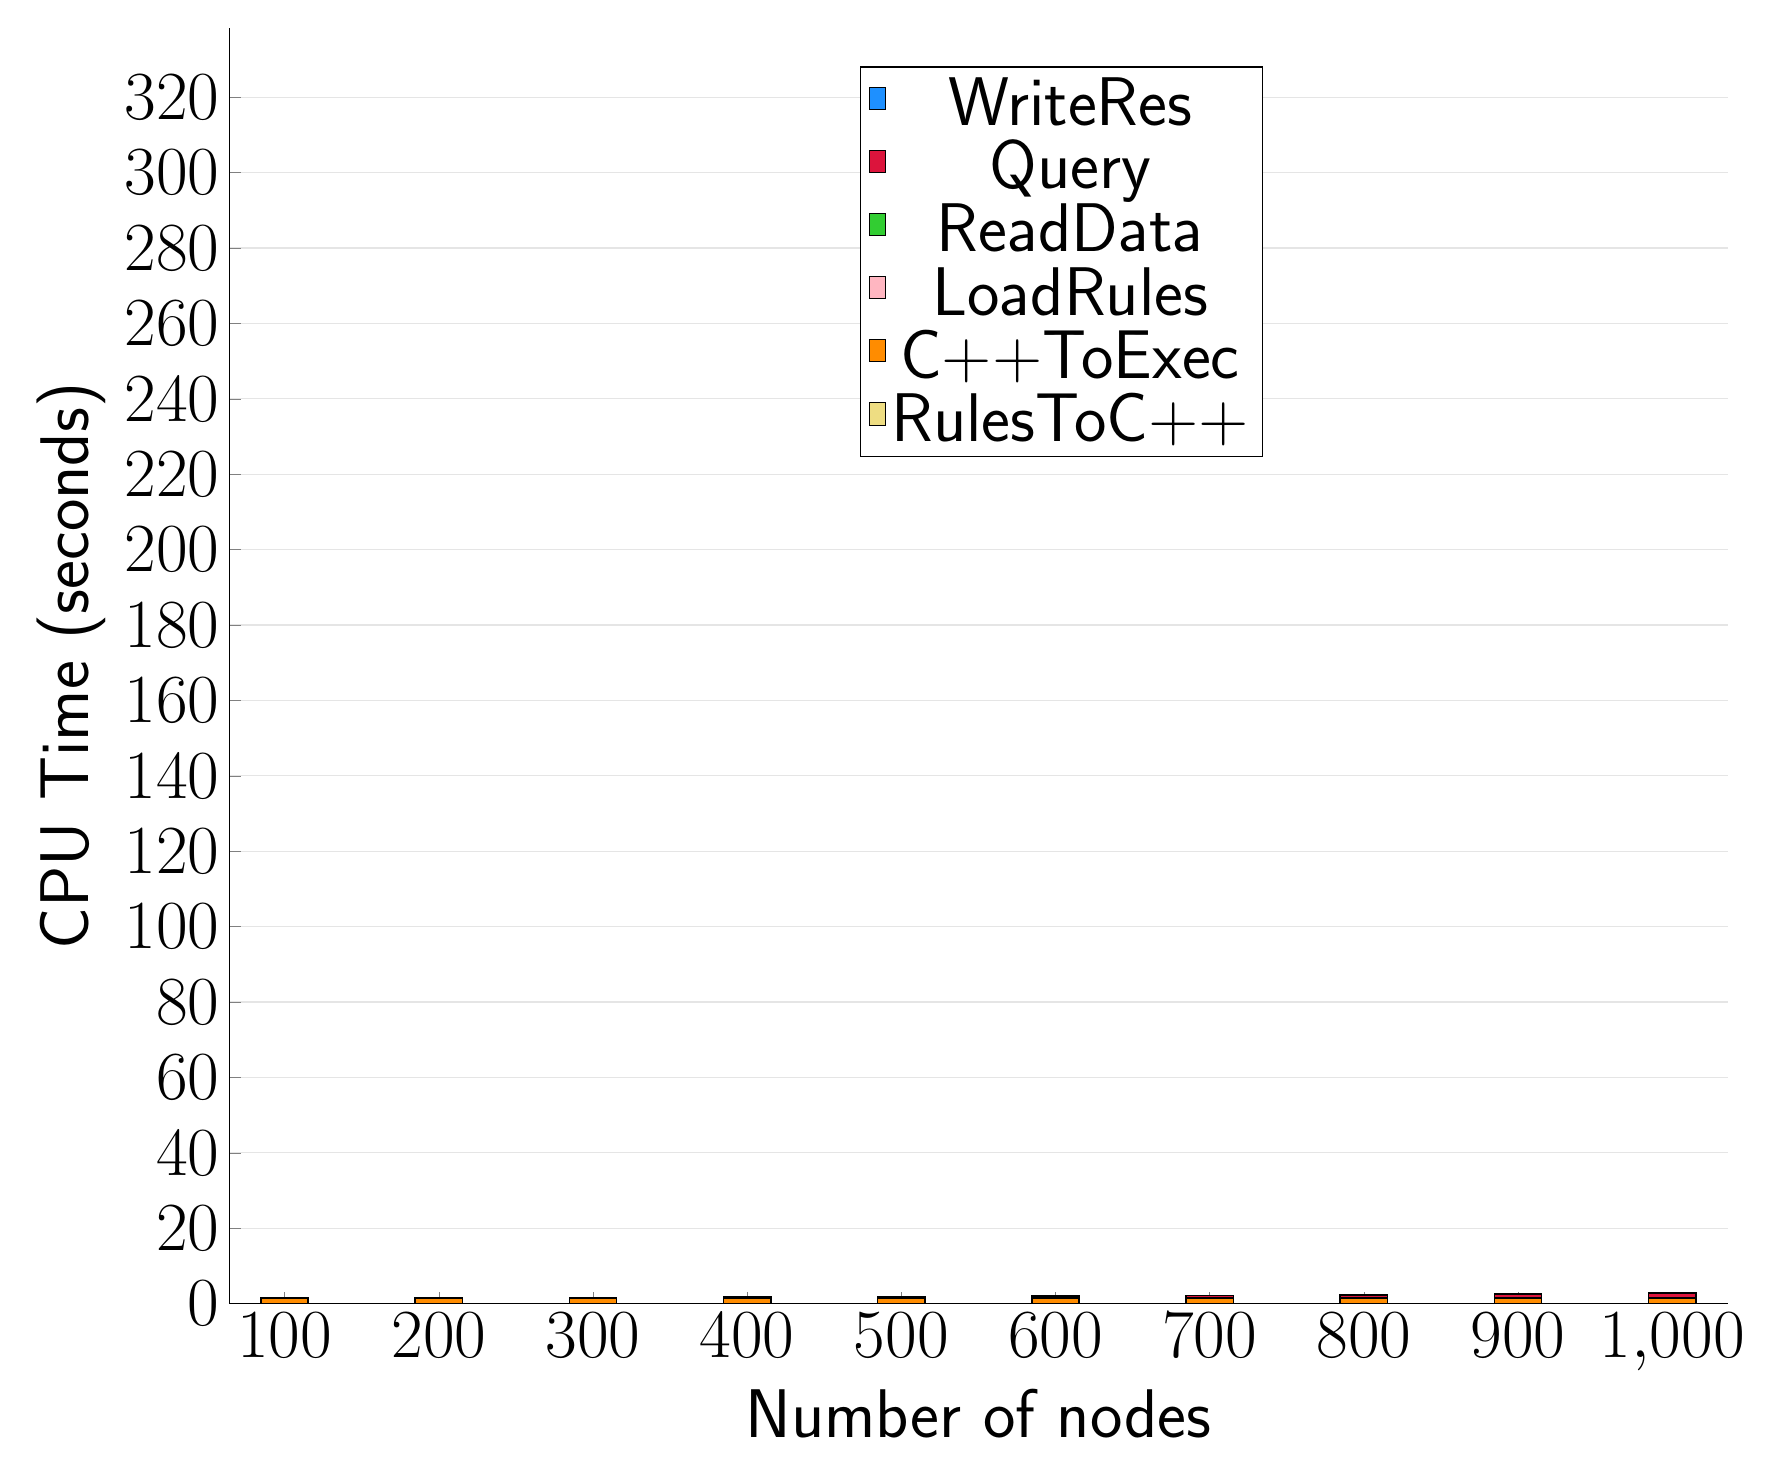
\begin{tikzpicture}
\begin{axis}[
   ybar stacked,
   width=1.7\textwidth,
   bar width=0.6cm,
   ymajorgrids, tick align=inside,
   major grid style={draw=gray!20},
   xtick=data,
   ymin=0, ymax=338.29920000000004,
   axis x line*=bottom,
   axis y line*=left,
   enlarge x limits=0.04,
   legend style={
       at={(0.69, 0.97)},
       anchor=north east,
       legend columns=1,
       font=\Huge,
   },
   ylabel={CPU Time (seconds)},
   xlabel={Number of nodes},
   label style={font=\Huge},
   tick label style={font=\Huge},
]
\addlegendimage{fill=DodgerBlue, draw=black, line width=0.2pt}
\addlegendentry{WriteRes}
\addlegendimage{fill=Crimson, draw=black, line width=0.2pt}
\addlegendentry{Query}
\addlegendimage{fill=LimeGreen, draw=black, line width=0.2pt}
\addlegendentry{ReadData}
\addlegendimage{fill=LightPink, draw=black, line width=0.2pt}
\addlegendentry{LoadRules}
\addlegendimage{fill=DarkOrange, draw=black, line width=0.2pt}
\addlegendentry{C++ToExec}
\addlegendimage{fill=LightGoldenrod, draw=black, line width=0.2pt}
\addlegendentry{RulesToC++}
\addplot +[fill=LightGoldenrod, draw=black, line width=0.55pt] coordinates {
(100, 0.0)
(200, 0.010000000000000002)
(300, 0.0020000000000000005)
(400, 0.006000000000000001)
(500, 0.004000000000000001)
(600, 0.010000000000000002)
(700, 0.008000000000000002)
(800, 0.010000000000000002)
(900, 0.004000000000000001)
(1000, 0.010000000000000002)
};
\addplot +[fill=DarkOrange, draw=black, line width=0.55pt] coordinates {
(100, 1.5240000000000002)
(200, 1.524)
(300, 1.532)
(400, 1.516)
(500, 1.52)
(600, 1.5119999999999998)
(700, 1.518)
(800, 1.5079999999999998)
(900, 1.518)
(1000, 1.51)
};
\addplot +[fill=LightPink, draw=black, line width=0.55pt] coordinates {
(100, 0.000151)
(200, 0.00014780000000000001)
(300, 0.00014800000000000002)
(400, 0.0001408)
(500, 0.00014560000000000002)
(600, 0.00010460000000000001)
(700, 0.0001402)
(800, 0.00013099999999999999)
(900, 0.00013739999999999998)
(1000, 0.0001602)
};
\addplot +[fill=LimeGreen, draw=black, line width=0.55pt] coordinates {
(100, 0.0008552000000000001)
(200, 0.001242)
(300, 0.0015164)
(400, 0.0019316)
(500, 0.0022638000000000003)
(600, 0.0022876)
(700, 0.0030514)
(800, 0.0029618)
(900, 0.0037606000000000002)
(1000, 0.004076000000000001)
};
\addplot +[fill=Crimson, draw=black, line width=0.55pt] coordinates {
(100, 0.0209554)
(200, 0.06425600000000001)
(300, 0.11915040000000002)
(400, 0.20050819999999997)
(500, 0.3086022)
(600, 0.4391328)
(700, 0.6013835999999999)
(800, 0.793763)
(900, 1.0096500000000002)
(1000, 1.260128)
};
\addplot +[fill=DodgerBlue, draw=black, line width=0.55pt] coordinates {
(100, 0.0002736)
(200, 0.0002464)
(300, 0.00021979999999999998)
(400, 0.0002636)
(500, 0.00026940000000000004)
(600, 0.0002934)
(700, 0.000289)
(800, 0.00031800000000000003)
(900, 0.00034619999999999996)
(1000, 0.0003562)
};
\end{axis}
\end{tikzpicture}

\end{document}
